\documentclass[12pt, a4paper]{article}

\usepackage[utf8]{inputenc}
\usepackage[T2A]{fontenc}
\usepackage[russian]{babel}
\usepackage{graphicx}
\usepackage[footnotesize]{caption2}
\usepackage{indentfirst}
\usepackage{titlesec}
\usepackage[]{placeins}

\usepackage[left=3cm,right=1.5cm,top=2.0cm,bottom=2.0cm,bindingoffset=0cm]{geometry}
\usepackage{pdfpages}
\usepackage[onehalfspacing]{setspace}
\onehalfspacing

\renewcommand{\baselinestretch}{1.1}
\renewcommand{\baselinestretch}{1.5} %для печати с большим интервалом

\newcommand{\sectionbreak}{\clearpage}
\renewcommand{\labelenumii}{\arabic{enumi}.\arabic{enumii}.}



\begin{document}
\sloppy
	
\begin{titlepage}
\newpage
		
\begin{figure}[t]
	\centering
	
\includegraphics[width=0.4\textwidth]{img/mgu}
\end{figure}
		
\begin{center}
Московский государственный университет имени М.В. Ломоносова \\
Факультет вычислительной математики и кибернетики \\
Кафедра автоматизации вычислительных комплексов \\
\end{center}
		
\vspace{4em}
\begin{center}
\large
Ермакова Татьяна Ивановна
\end{center}
	
\begin{center}
\Large
\bfseries
Метод и средства передачи данных в реальном времени в программно-конфигурируемых сетях
\end{center}

\vspace{3em}
\begin{center}
\large
\textsc{
	магистерская диссертация
}
\end{center}

\vspace{5em}
\begin{flushright}
	\textbf{Научный руководитель:}\\
	к.ф.-м.н с.н.с\\
	В.В.Балашов\\
\end{flushright}%


\vspace{\fill}
\begin{center}
Москва 2019
\end{center}
		
\end{titlepage}

\section*{Аннотация}
В данной работе реализован предложенный автором подход к передаче данных в условиях реального времени в программно-конфигурируемых сетях (ПКС). Подход основан на схеме управления трафиком в ПКС, описанной в предыдущих работах автора, и предложенном в данной работе алгоритме реконфигурации систем виртуальных каналов. Алгоритм реконфигурации основан на жадных стратегиях и позволяет произвести восстановление работы системы, минимизируя время простоя и количество изменений в таблицах коммутации. Реализация подхода выполнена в виде программного средства, выполняющего функции мониторинга сети и её реконфигурации в случае возникновения сбоев с использованием предложенных алгоритма и схемы. Программное средство представляет собой приложение для ПКС-контроллера RUNOS. Проведённое экспериментальное исследование продемонстрировало работоспособность предложенного подхода и входящего в него алгоритма реконфигурации в условиях реального времени.

\renewcommand{\contentsname}{Содержание}
\tableofcontents

\section*{Введение}
\addcontentsline{toc}{section}{Введение}
Специфика передачи данных в вычислительных системах реального времени (ВС РВ) заключается в повышенных требованиях к надежности и наличии жестких ограничений на время выполнения обмена сообщениями между абонентами. При построении ВС РВ предпочтение отдается коммутируемым средам обмена, которые в отличие от каналов вида точка-точка позволяют сократить число физических кабелей и гибко распределить пропускную способность.

Для избегания конфликтов между потоками данных в коммутируемых средах обмена используется механизм виртуальных каналов. Для удовлетворения потребностей ВС РВ при помощи этого механизма к виртуальным каналам предъявляются требования на ограничение следующих характеристик:
\begin{itemize}
	\item пропускной способности;
	\item задержки передачи данных;
	\item флуктуации задержки (джиттера).
\end{itemize}

Выполнение данных требований обеспечивается назначением виртуальным каналам ряда параметров, состав которых зависит от используемой схемы построения ВС РВ. Параметры виртуальных каналов в совокупности с их маршрутами образуют конфигурацию системы. Существуют следующие стандарты построения коммутируемых сетей ВС РВ на основе виртуальных каналов:
\begin{enumerate}
	\item Avionics Full Duplex Ethernet (AFDX) \cite{afdx}.
	\item FC-AE-ASM-RT на основе Fibre Channel \cite{fcaert}.
\end{enumerate}

Недостатком данных решений является статичность системы виртуальных каналов. Существующие стандарты предусматривают наличие ограниченного набора заранее заданных конфигураций, изменение которого невозможно в ходе работы ВС РВ. Переключение между такими конфигурациями не дает возможности гибко реагировать на сбои в работе системы.

Решением данной проблемы могут служить программно-конфигурируемые сети (ПКС) \cite{sdn}. ПКС является перспективным видом компьютерных сетей, главной особенностью которых являются широкие возможности реконфигурации. Использование ПКС для передачи данных в реальном времени даст возможность производить расчет и применение новых конфигураций сети в ходе работы системы. Это позволит перераспределять потоки данных при возникновении сбоев или смене режима работы. На текущий момент не существует готовых решений, допускающих использование ПКС в составе ВС РВ при контроле полного состава параметров управления трафиком, принятых для сетей на основе виртуальных каналов.

Данная работа посвящена созданию методов и средств, позволяющих использовать ПКС в системах реального времени с учётом предъявляемых требований качества обслуживания.

\section{Постановка задачи}
Целью работы является разработка подхода к использованию программно-конфигурируемых сетей в составе вычислительных реального времени. В основу подхода положена ранее разработанная автором схема управления потоками данных в ПКС на основе виртуальных каналов \cite{vlsdn}. Для достижения этой цели должны быть решены следующие задачи:
\begin{enumerate}
	\item Разработка алгоритма динамической реконфигурации виртуальных каналов.
	\item Реализация приложения для контроллера ПКС, выполняющего функции мониторинга сети и её реконфигурации при выявлении отказов на основе предложенного алгоритма.
	\item Экспериментальное исследование полученного решения по критерию работоспособности в условиях реального времени.
\end{enumerate}

\section{Управление трафиком в ВС реального времени с использованием виртуальных каналов} \label{sec:scheme}
\subsection{Схема управления трафиком}
В основе подхода, описанного в \cite{vdovin} и используемого в сетях AFDX \cite{afdx}, FC-AE-ASM-RT \cite{fcaert}, а также в ранее предложенной автором схеме управления трафиком в  ПКС, лежит согласованная работа оконечных систем (абонентов) и коммутаторов:
\begin{itemize}
	\item Оконечные системы при помощи планировщика обеспечивают корректную выдачу данных в сеть. Планировщик на каждой оконечной системе формирует трафик для виртуальных каналов и мультиплексирует их для выдачи на физическую линию.
	\item Коммутатор осуществляет контроль трафика при помощи алгоритма текущего ведра независимо для каждого виртуального канала. При превышении заданной пропускной способности кадры данного канала начинают сбрасываться.
\end{itemize}


Для алгоритма текущего ведра вводится ряд параметров виртуального канала:
\begin{itemize}
	\item BAG -- минимальный интервал времени вежду началами выдачи последовательных кадров на данном виртуальном канале.
	\item $L_{max}$ -- максимальная длина передаваемого кадра.
	\item $J_{max}$ -- джиттер, максимальная задержка от начала временного слота до начала передачи кадра.
\end{itemize}

Для контроля трафика вводится кредит на количество передаваемых байт, максимальное значение которого равно $AC_{max} = L_{max}(1 + \frac{J_{max}}{BAG})$. Значение
кредита увеличивается с течением времени пропорционально величине $\frac{L_{max}}{BAG}$.

При поступлении кадра (или пакета) значение кредита уменьшается на его размер в случае, если этот размер не превосходит значения кредита. Иначе кадр (пакет) сбрасывается. Такая схема позволяет контролировать пропускную способность и джиттер. Работа алгоритма показана на рисунках~\ref{pic:scheme:nojit} и~\ref{pic:scheme:jit}.

\begin{figure}[h!]
	\centering
	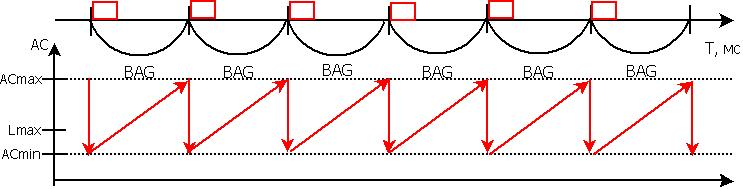
\includegraphics[width=0.80\textwidth]{img/nojit.png}
	\caption[russian]{Работа алгоритма текущего ведра при нулевом джиттере.}
	\label{pic:scheme:nojit}
\end{figure}

\begin{figure}[h!]
	\centering
	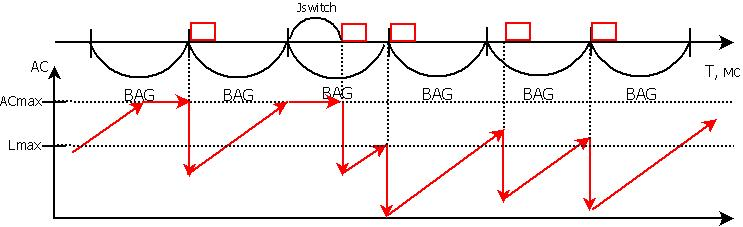
\includegraphics[width=0.80\textwidth]{img/jit.png}
	\caption{Работа алгоритма текущего ведра при ненулевом джиттере.}
	\label{pic:scheme:jit}
\end{figure}
\FloatBarrier

\subsection{Реализации схемы управления трафиком}
В данном разделе описываются индивидуальные особенности следующих схем управления трафиком:
\begin{itemize}
	\item AFDX.
	\item FC-AE-ASM-RT.
	\item Предложенная ранее автором схема управления трафиком в ПКС.
\end{itemize}

Стандарты AFDX и FC-AE-ASM-RT определяют построение сетей ВС РВ на основе виртуальных каналов. Маршрутизация в таких сетях производится коммутаторами при помощи статических таблиц, которые настраиваются заранее. Контроль трафика осуществляется с использованием алгоритма текущего ведра на уровне кадров. Алгоритм встроен в специализированные коммутаторы этих сетей.

В ПКС маршрутизация производится коммутаторами на основе динамических таблиц, задаваемых контроллером. Предложенная автором схема, описанная в \cite{vlsdn}, основывается на механизме meter-таблиц \cite{meter}, показанных на рисунке~\ref{pic:scheme:meter} и являющихся частью стандарта OpenFlow1.3 \cite{openflow}. Такие таблицы также управляются контроллером и могут быть изменены в процессе работы системы. Каждая запись meter-таблицы задаёт измеритель, контролирующий скорость привязанных к нему потоков. Схема, по которой осуществляется данный контроль, не закреплена в стандарте и зависит от конкретных реализаций. 

\begin{figure}[h!]
	\centering
	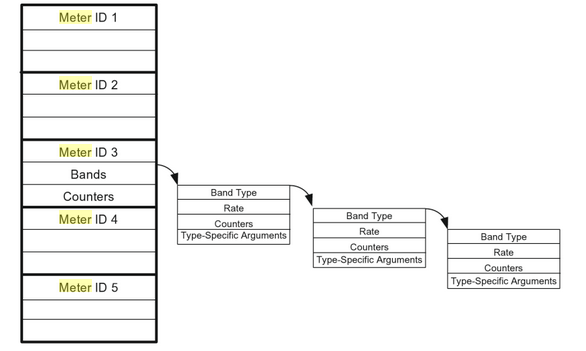
\includegraphics[width=0.80\textwidth]{img/meter.png}
	\caption{Структура meter-таблицы.}
	\label{pic:scheme:meter}
\end{figure}

Программный коммутатор Ofsoftswitch13 \cite{ofsoftswitch} реализует контроль трафика измерителями при помощи алгоритма текущего ведра и поэтому лег в основу предложенной автором схемы управления трафиком в ПКС.

Схема управления трафиком заключается в следующем:
\begin{itemize}
	\item Для каждого потока задается свой измеритель, на который средствами OpenFlow, посылается максимальное значение кредита и скорость его роста.
	\item Проверка допустимости трафика производится при помощи алгоритма текущего ведра отдельно для каждого потока на уровне пакетов.
\end{itemize}

\subsection{Сравнение реализаций по критерию поддержки реконфигурируемости} \label{subsec:reconf}
Конфигурацией сети на основе виртуальных каналов назовем набор параметров виртуальных каналов в совокупности с их маршрутами. Каждой конфигурации соответствует набор таблиц маршрутизации, определяющих действия коммутаторов по передаче данных и контролю трафика в соответствии с данной конфигурацией.

Стандарт AFDX предусматривает наличие одной фиксированной таблицы маршрутизации на каждом коммутаторе. Такой набор таблиц маршрутизации соответствует единственной доступной в сети AFDX конфигурации.

Стандарт FC-AE-ASM-RT имеет возможность поддерживать на коммутаторах несколько таблиц маршрутизации, задаваемых до начала работы системы. Это позволяет задать несколько конфигураций сети. Переход между такими конфигурациями осуществляется при помощи контроллера конфигураций. Им является дополнительная оконечная станция. При смене конфигурации контроллер сообщает коммутаторам сети идентификатор новой конфигурации. На каждом коммутаторе находится внутренняя оконечная станция, обрабатывающая информацию о смене конфигурации. Так как контроллером передается только идентификатор, весь набор конфигураций должен быть заложен в коммутаторы до начала работы системы. На время процесса перехода, который может длиться до 40 мс, все коммуникации в системе временно приостанавливаются, так как происходит полная смена таблиц коммутации. Таким образом процесс смены конфигурации нарушает циркуляцию трафика всех потоков данных системы.

В ПКС таблицы коммутаторов управляются контроллером при помощи сообщений, регламентируемых протоколом OpenFlow. В предложенной автором схеме модификация параметров виртуальных каналов производится сообщениями FlowMod и MeterMod протокола OpenFlow1.3. За счёт этого таблицы маршрутизации, равно как и meter-таблицы, могут быть изменены любым образом в ходе работы системы. Это позволяет создавать множество конфигураций, размер которого ограничен лишь возможностями физической среды передачи данных. Процесс изменения таблиц коммутаций не затрагивает абсолютно все, содержащиеся в них правила. Это даёт возможность не нарушать движение трафика по виртуальным каналам, маршруты которых не проходили через элементы сети, попавшие под сбой. Для виртуальных каналов, пути следования которых были подвержены поломке, имеется возможность сохранить часть пакетов в случае совпадения участков старого и нового маршрутов. 

Динамическая реконфигурация сетей ВСРВ требуется в случаях:
\begin{enumerate}
	\item смены режимов работы;
	\item выхода из строя вычислителей.
\end{enumerate}

Как было показано выше стандарт AFDX не поддерживает реконфигурацию в ходе работы системы. Возможностей же FC-AE-ASM-RT недостаточно для произведения гибкой реконфигурации, так как все сбойные режимы должны быть заранее заложены в у. Для единичного отказа число таких режимов является достаточно большим и оценивается количеством физических элементов сети. Расчет всех случаев множественного отказа является ещё более нетривиальной задачей, а хранение всех таких конфигураций в памяти коммутаторов не представляется возможным. Использование ПКС в ВС РВ позволяет производить расчет и применение новой конфигурации сети непосредственно при возникновении поломки. Такой вариант реконфигурации позволяет системе частично продолжать функционировать даже в процессе перехода. Всё это даёт возможность гибко реагировать на множественные сбои и восстанавливать работу системы в полном объеме в тех случаях, когда это позволяют физические ресурсы.


\section{Актуальность задачи}
Динамическая реконфигурация сети востребована в ВС РВ, как было показано в разделе~\ref{subsec:reconf}. Возможность перераспределить потоки данных в ходе работы системы необходима при возникновении сбоев или желании заложить несколько режимов работы в систему. Существующее решение, предложенное в \cite{fakevlsdn}, не описывает схему контроля параметров качества обслуживания и представлено, как альтернатива дублированию сети, обеспечивающая восстановление работы системы в случаях единичных сбоев. 

В разделе \ref{sec:scheme} было продемонстрировано, что в ПКС имеются возможности для гибкой реконфигурации сети при соблюдении требований к качеству обслуживания, принятых в сетях ВС РВ. Для осуществления реконфигурации в случае возникновения сбоев необходимо:
\begin{enumerate}
	\item Определить, в какой части сети произошел сбой.
	\item Произвести расчет новой конфигурации с учетом вышедших из строя элементов сети.
	\item Произвести переход на полученную конфигурацию.
\end{enumerate}

Данная работа посвящена алгоритму расчета новой конфигурации сети, а также его реализации в составе средства мониторинга и реконфигурации ПКС в условиях реального времени. Также в работе описан и реализован процесс идентификации сбоев. Процедура смены конфигураций ранее была реализована и апробирована в рамках подтверждения работоспособности схемы управления трафиком в ПКС.

\section{Алгоритм реконфигурации виртуальных каналов} \label{sec:alg}
\subsection{Общая схема алгоритма}

В процессе разработки алгоритма реконфигурации был изучен ряд работ, посвященных построению маршрутов систем виртуальных каналов addlinks. Во всех перечисленных работах формирование конфигурации ведётся при помощи последовательного применения процедуры поиска маршрута к каждому из виртуальных каналов с использованием жадных стратегий.

В основу предлагаемого алгоритма лёг описанный в работе \cite{vdovinalg} подход к построению систем виртуальных каналов для сетей AFDX. Однако этот подход не может быть позаимствован целиком, так как применяется для начальной инициализации сети и не удовлетворяет ограничениям, накладываемым в данной работе. Разрабатываемый алгоритм реконфигурации систем виртуальных каналов функционирует в условиях реального времени, а потому должен быть направлен на минимизацию:
\begin{itemize}
	\item времени расчёта новой конфигурации;
	\item времени применения новой конфигурации в сети, а значит и количества изменений в таблицах коммутации;
	\item числа пакетов, потерянных в процессе реконфигурации.
\end{itemize} 

Для достижения этих целей алгоритм разделён на два этапа -- базовый и дополнительный. На базовом этапе рассматриваются только те виртуальные каналы, которые необходимо переложить, так как они проходят через сбойные элементы сети. В случае если невозможно произвести реконфигурацию, рассматривая только это множество виртуальных каналов, для восстановления работы сети производится дополнительный этап, на котором затрагивается более широкое множество виртуальных каналов. Общая схема алгоритма показана на рисунке~\ref{pic:algorithm}

\begin{figure}[h!]
	\centering
	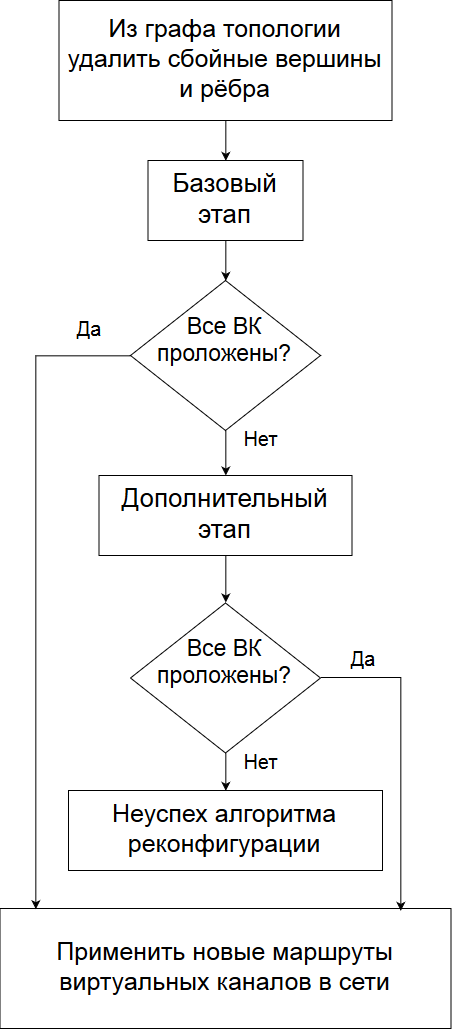
\includegraphics[width=0.50\textwidth]{img/alg.png}
	\caption{Общая схема алгоритма реконфигурации.}
	\label{pic:algorithm}
\end{figure}


Применение новых маршрутов в сети осуществляется только после успешного завершения работы алгоритма. Поведение приложения реконфигурации при неуспешном завершении алгоритма в рамках данной работы не рассматривается. Однако предполагается, что в этом случае будет предпринята попытка переложить часть виртуальных каналов в зависимости от их приоритета. Приоритет виртуального канала в такой модели будет определяться исходя из критичности наличия потока данных для работы системы.  

\FloatBarrier

\subsection{Процедуры поиска нового маршрута виртуального канала} \label{subsec:procalg}
В основе каждого этапа алгоритма реконфигурации лежит поиск нового маршрута виртуального канала, который может осуществляться несколькими способами. Опишем эти способы прежде, чем приступить к описанию этапов алгоритма.

Введём обозначения:
\begin{itemize}
	\item $S$ -- узел-отправитель для данного виртуального канала.
	\item $R$ -- узел-получатель для данного виртуального канала.
	\item $Node_{S}$ – один из узлов, между которыми прервалась связь, ближний к $S$.
	\item $Node_{R}$ – один из узлов, между которыми прервалась связь, ближний к $R$.
\end{itemize}

Процедуры поиска нового маршрута виртуального канала основываются на жадных стратегиях. Их отличие между собой заключается в глубине и скорости поиска. На базовом этапе алгоритма будет выполнен более быстрый вариант процедуры, так как цель базового этапа попытаться произвести реконфигурацию за как можно более короткий срок.

Первый вариант процедуры поиска:
\begin{enumerate}
	\item Используя алгоритм Дейкстры \cite{dejkstra}, найти кратчайший путь между $Node_{S}$ и $R$.
	\item Добавить в него путь от $S$ к $Node_{S}$.
	\item Удалить циклы.
\end{enumerate}

Такая процедура поиска позволяет сохранить участок пути от $S$ к $Node_{S}$, когда это возможно. За счёт этого часть пакетов, отправляемых в процессе реконфигурации, не будет потеряна и будет перенаправлена по новому маршруту от $Node_{S}$ к $R$. Процедура направлена на минимизацию потерь, возникающих во время построения и применения новой конфигурации.

Второй вариант процедуры поиска:
\begin{enumerate}
	\item Используя алгоритм k-кратчайших путей \cite{kshort}, найти кратчайший путь между $S$ и $R$.
	\item Выбрать путь по критерию совпадения наибольшего со старым маршрутом.
\end{enumerate}

Второй вариант процедуры даёт возможность найти большее количество альтернативных маршрутов. Для ограничения глубины поиска было выбрано значение $k = 3$. Ограничение на сохранение участка пути от $Node_{S}$ к $R$ снимается, но при этом выбор итогового маршрута зависит от исходного маршрута виртуального канала, что позволяет минимизировать число изменений в таблицах коммутации.

\subsection{Описание базового этапа алгоритма}

На данном этапе производится попытка найти новые маршруты для виртуальных каналов, проходивших через сбойные элементы сети. Остальные виртуальные каналы при этом не затрагиваются. Такой подход при успешном завершении данного этапа позволяет произвести реконфигурацию с минимальными изменениями в сети. Ограниченный набор обрабатываемых виртуальных каналов и быстрая процедура поиска нового маршрута дают возможность минимизировать время работы базового этапа.

Обозначим за $(A)$ набор виртуальных каналов, проходивших через отказавший элемент сети. Пропускная способность вычисляется из параметров виртуального канала, описанных в разделе~\ref{sec:scheme} и равна:
$$bw = \frac{L_{max}}{BAG}$$

Базовый этап алгоритма реконфигурации:
\begin{enumerate}
	\item Для каждого виртуального канала из набора $(A)$ в порядке убывания пропускной способности выполнить:
	\begin{enumerate}
	\item Удалить все ребра, на которых не хватает пропускной способности для данного виртуального канала.
	\item Запустить первый вариант процедуры поиска нового маршрута виртуального канала, описанный в разделе~\ref{subsec:procalg}.
	\item В случае неуспеха перейти к пункту 2.
	\item Актуализировать значения пропускных способностей в графе сети с учётом построенного маршрута.
	\end{enumerate}
	\item Завершить этап.
\end{enumerate}

\subsection{Описание дополнительного этапа алгоритма}
На данном этапе задействуется более широкий набор виртуальных каналов, чем на базовом этапе. Сначала осуществляется перепрокладка всех виртуальных каналов, проходивших через сбойные элементы сети. Это позволяет изменить ситуацию в сети и найти новые маршруты для нарушенных виртуальных каналов. Более глубокая процедура поиска нового маршрута, используемая на данном этапе, также способствует вычислению доступной конфигурации сети. Целью данного этапа является осуществить реконфигурацию, несмотря на то, что неуспех базового этапа показал сложность данной процедуры.

Пусть $bw_{max}$ -- максимальная пропускная способность виртуальных каналов из множества $(A)$.
Обозначим за $(B)$ подмножество всех виртуальных каналов, которые не входят в $(A)$ и пропускная способность которых не больше $bw_{max}$.

Дополнительный этап алгоритма реконфигурации:
\begin{enumerate}
	\item Для каждого виртуального канала из набора $(A)$ в порядке убывания пропускной способности выполнить:
	\begin{enumerate}
		\item Удалить все ребра, на которых не хватает пропускной способности для данного виртуального канала.
		\item Запустить второй вариант процедуры поиска нового маршрута виртуального канала, описанный в разделе~\ref{subsec:procalg}.
		\item В случае неуспеха перейти к пункту 3.
		\item Актуализировать значения пропускных способностей в графе сети с учётом построенного маршрута.
	\end{enumerate}
	\item Для каждого виртуального канала из набора $(B)$ в порядке убывания пропускной способности выполнить:
	\begin{enumerate}
		\item Удалить все ребра, на которых не хватает пропускной способности для данного виртуального канала.
		\item Запустить второй вариант процедуры поиска нового маршрута виртуального канала, описанный в разделе~\ref{subsec:procalg}.
		\item В случае неуспеха перейти к пункту 3.
		\item Актуализировать значения пропускных способностей в графе сети с учётом построенного маршрута.
	\end{enumerate}
	\item Завершить этап.
\end{enumerate}


\section{Структура и функции приложения реконфигурации}
\subsection{Назначение и структура приложения реконфигурации}

Приложение реконфигурации для ПКС-контролера, реализующего предлагаемый подход, должно:
\begin{itemize}
	\item реализовывать функции мониторинга для обнаружения сбоев;
	\item реализовывать функции реконфигурации при возникновении сбоев, а именно расчета новой конфигурации и её применения в сети;
	\item производить расчет новой конфигурации с использованием алгоритма, предложенного в разделе~\ref{sec:alg};
	\item применять изменения в сети на основе схемы, описанной в разделе~\ref{sec:scheme}.
\end{itemize}

Общая структура приложения реконфигурации, разработанного автором, показана на рисунке~\ref{pic:netcontrol}.

\begin{figure}[h!]
	\centering
	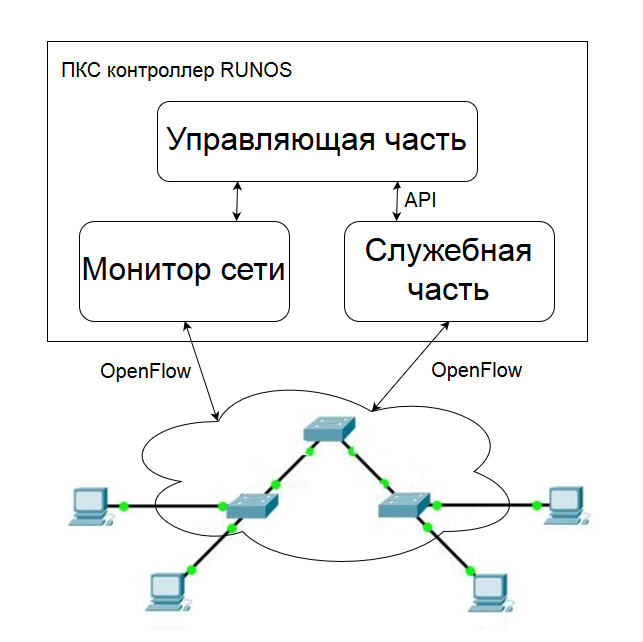
\includegraphics[width=0.80\textwidth]{img/netcontrol.png}
	\caption{Структура приложения реконфигурации.}
	\label{pic:netcontrol}
\end{figure}


\subsection{Описание функций служебной части}
Служебная часть реализует в себе описанную в разделе~\ref{sec:scheme} схему управления трафиком в ПКС на основе виртуальных каналов.
 
Служебная часть должна предоставлять управляющей:
\begin{itemize}
	\item информацию о потоках данных, которыми обмениваются абоненты сети;
	\item информацию о проложенных в сети виртуальных каналах и их параметрах;
	\item интерфейс для добавления/удаления/модификации виртуальных каналов с определенными параметрами качества обслуживания.
\end{itemize}

\subsection{Описание функций управляющей части}
Управляющая часть реализует в себе описанный в разделе~\ref{sec:alg} алгоритм реконфигурации систем виртуальных каналов.

Управляющая часть:
\begin{itemize}
	\item отвечает за построение начальных маршрутов виртуальных каналов;
	\item отвечает за построение новых маршрутов виртуальных каналов при выходе из строя компонентов сети;
	\item использует API служебной части для применения новых маршрутов в сети после завершения работы алгоритма реконфигурации;
	\item использует информацию, полученную от монитора, для инициализации алгоритма реконфигурации.
\end{itemize}

\subsection{Описание функций монитора}

Процедура мониторинга содержит в себе три составляющие:
\begin{enumerate}
	\item Мониторинг состояния коммутаторов.
	\item Мониторинг состояния физических линий связи.
	\item Мониторинг состояния оконечных систем.
\end{enumerate}

Мониторинг состояний коммутаторов и физических соединений между коммутаторами производится стандартным для ПКС способом, описанным в \cite{monitor1, monitor2}. Ниже приведено краткое описание этих процедур. В силу специфики задачи, а именно необходимости совместной работы отправителей и коммутаторов, работа оконечных систем может быть предопределена. Особенности их функционирования задаются в момент проектирования системы. Поэтому на них может быть возложена функция отправки диагностических пакетов. Это позволяет использовать схему мониторинга состояния оконечных систем, в которой нагрузки на сеть данных ниже в сравнении с со стандартной схемой.

Мониторинг состояния коммутаторов производится на уровне OpenFlow при помощи сообщений EchoReq и EchoRes. Раз в период коммутатор и контроллер обмениваются ими для подтверждения живости друг друга.

Мониторинг состояния оконечных систем производится по следующей схеме:
\begin{enumerate}
	\item Оконечная система раз в период посылает пакет на ближайшие коммутаторы.
	\item На коммутаторах инициируется сообщение Packet-in, сообщающее контроллеру о поступлении неизвестного пакета.
	\item Контроллер, не получив раз в период ни одного Packet-in, в котором в поле отправителя содержится идентификатор данной оконечной системы, считает её отключённой.
\end{enumerate}


Процедуру мониторинга состояния физических линий можно разделить на две составляющие: 
\begin{itemize}
	\item мониторинг линий между коммутаторами;
	\item мониторинг линий между коммутаторами и оконечными системами.
\end{itemize}

Физическая линия считается из строя в случае если с коммутатора поступило сообщение, свидетельствующее об отключении соответствующего порта. В рамках OpenFlow для этого используется сообщение PortStatus, его отправка инициируется самим коммутатором при изменении статуса порта.

Мониторинг линии между коммутаторами осуществляется на основе протокола Link Layer Discovery Protocol (LLDP), описанного в \cite{monitor2}, следующим образом:
\begin{enumerate}
	\item Контроллер отправляет инкапсулированный в Packet-out LLDP-пакет на соответствующий порт коммутатора. В Packet-out содержится информация о пересылке LLDP-пакета по исследуемой физической линии.
	\item Коммутатор отправляет LLDP-пакет по линии на другой коммутатор.
	\item Второй коммутатор, получив LLDP-пакет, инкапсулирует его в Packet-In и отправляет контроллеру.
	\item Получив обратно пакет, контроллер делает вывод о живости физической линии.
\end{enumerate}

Мониторинг линий между коммутаторами и оконечными системами производится совместно с мониторингом самих оконечных систем. Разница заключается в том, что каждый Packet-in отвечает за свою физическую линию.

Монитор сети реализует описанную схему мониторинга, а также:
\begin{itemize}
	\item отвечает за построение начальной топологии сети;
	\item сообщает управляющей части о выходе из строя компонентов сети.
\end{itemize}

\section{Программная реализация}
\subsection{Выбор базового программного обеспечения сети}

В данном разделе обосновывается выбор коммутаторов и контроллера, используемых в предлагаемом подходе и дальнейших исследованиях.

Выбор коммутаторов основывается на используемой схеме управления трафиком. При этом к коммутаторам предъявляются следующие требования:
\begin{itemize}
	\item Поддержка механизма meter-таблиц.
	\item OpenFlow не ниже 1.3.
	\item Реализация механизма meter-таблиц должна основываться на алгоритме текущего ведра.
\end{itemize}

Корректность схемы управления трафиком в ПКС с использованием программного коммутатора Ofsoftswitch13 \cite{ofsoftswitch} была подтверждена в предыдущих работах автора. Поэтому выбор сделан в его пользу.

Выбор контроллера обусловлен следующими критериями:
\begin{itemize}
	\item Язык реализации С++, который обеспечивает более детерминированное время работы. Обоснование этому может быть найдено в \cite{cpp}.
	\item OpenFlow версии не ниже 1.3
	\item Поддерживаемость ?? add как сказать лучше.
\end{itemize}

Были рассмотрены следующие варианты контроллеров, реализованных на C++: NOX \cite{nox} и RUNOS \cite{runos}. Контроллер NOX больше не поддерживается разработчиками, тогда как RUNOS активно развивается, поэтому выбор был сделан в пользу второго.

\subsection{Структура программного средства}
Диаграмма, отражающая основные программные компоненты приложения реконфигурации показана на рисунке~\ref{pic:classes}. Реализация выполнена на языке C++.

\begin{figure}[h!]
	\centering
	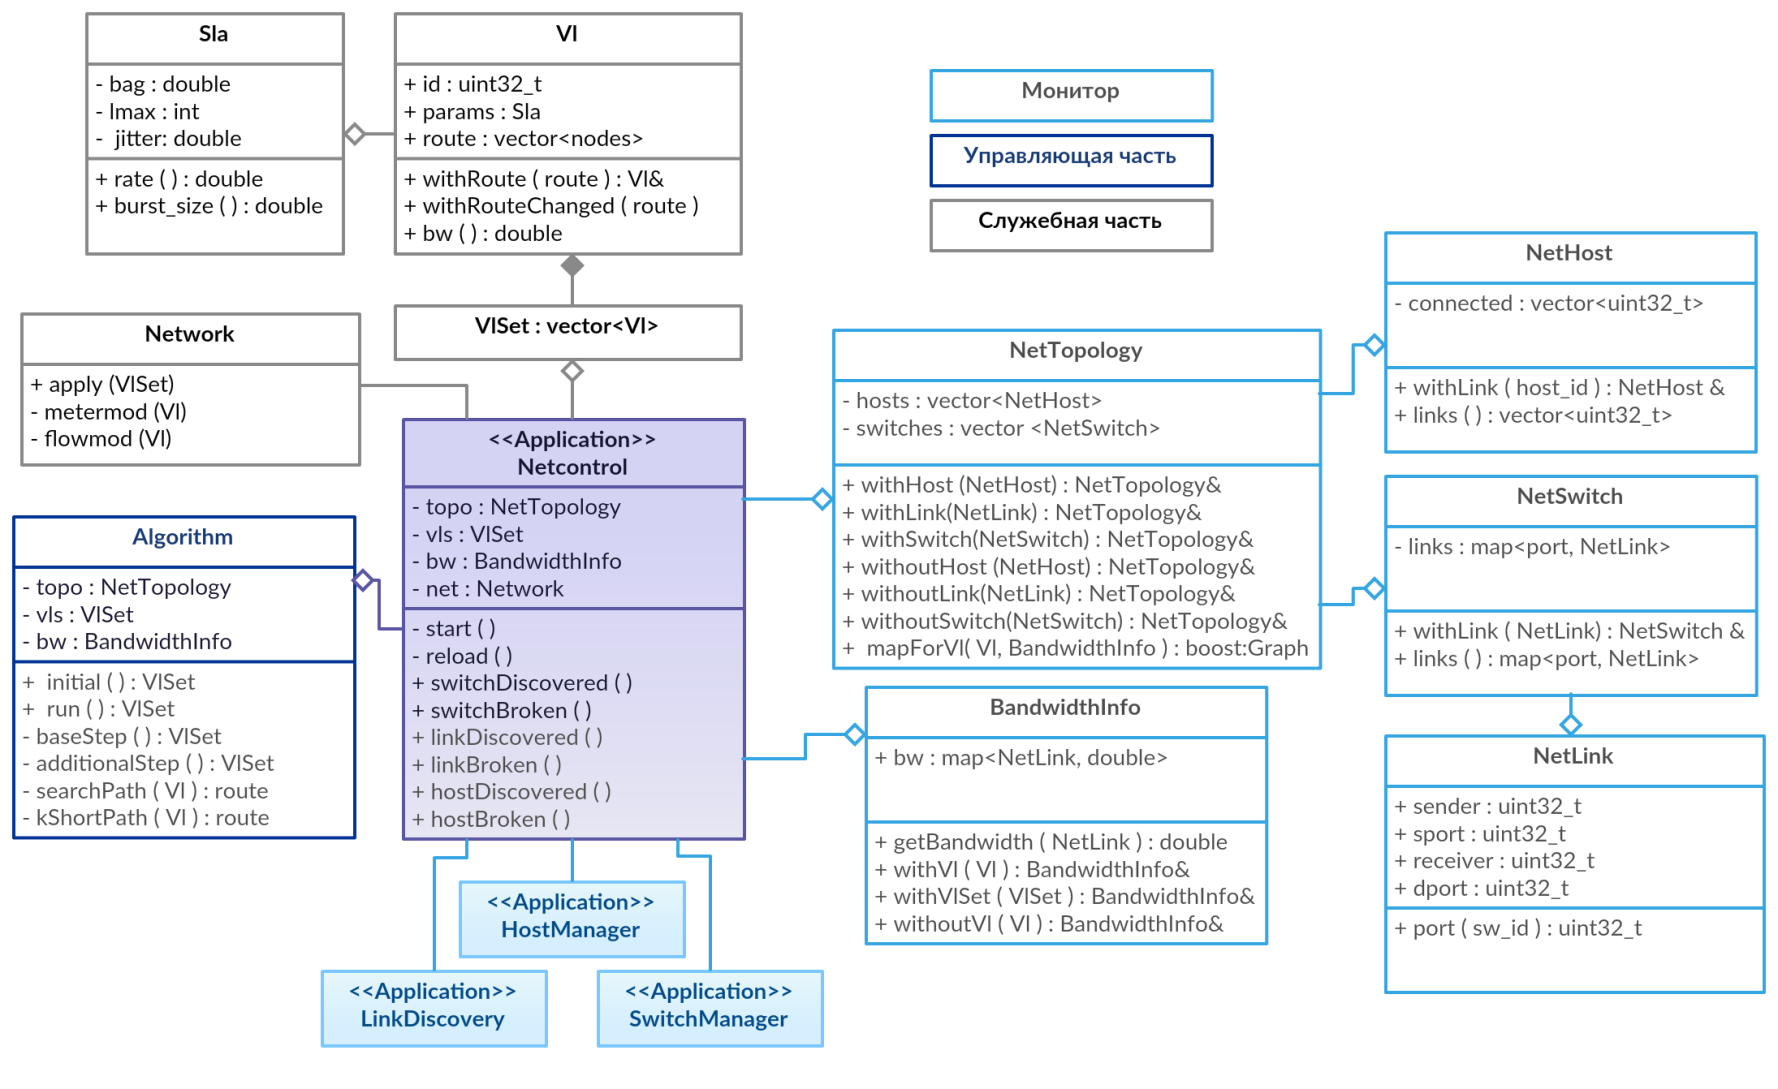
\includegraphics[width=0.80\textwidth]{img/classes.png}
	\caption{Основные классы программной реализации.}
	\label{pic:classes}
\end{figure}


Основные программные компоненты служебной части:
\begin{itemize}
	\item Sla - класс характеристик виртуальных каналов.
	\item Vl - класс, отвечающий за хранение параметров виртуальных каналов (включая их маршруты).
	\item VlSet - набор виртуальных каналов.
	\item Network - интерфейс для применения настроек виртуальных каналов. Формирует набор сообщений для применения соответствующих параметров и маршрутов в сети.
\end{itemize}

Основные программные компоненты управляющей части:
\begin{itemize}
	\item Netcontrol - класс, отвечающий за запуск алгоритма реконфигурации и обработку данных, полученных от монитора. Является классом приложения Runos.
	\item Algorithm - класс, реализующий алгоритмы построения маршрутов виртуальных каналов.
\end{itemize}

Основные программные компоненты монитора:
\begin{itemize}
	\item NetTopology - класс, отображающий текущее состояние топологии сети. Использует вспомогательные классы NetLink, NetSwitch и NetHost для хранения информации о каналах, коммутаторах и абонентах соответственно.
	\item BandwidthInfo - хранит текущую доступную на физических каналах пропускную способность. Начальные значения задаются в конфигурации приложения.
	\item HostManager - приложение Runos, анализирующее состояние абонентов. Приложение написано автором работы.
	\item SwitchManager - приложение Runos, анализирующее состояние коммутаторов. Используется стандартное приложение, входящее в состав контроллера.
	\item LinkDiscovery - приложение Runos, анализирующее состояние физических каналов. Используется стандартное приложение, входящее в состав контроллера.
\end{itemize}


\section{Экспериментальное исследование}
\subsection{Цель исследования}
Целью исследования является анализ характеристик и подтверждение работоспособности в реальном времени предложенного в работе алгоритма реконфигурации виртуальных каналов, предназначенного для использования в рамках описанного подхода к передаче данных в ПКС в условиях реального времени. Для достижения поставленной цели необходимо:
\begin{itemize}
	\item провести исследование свойств алгоритма на различных классах входных данных; 
	\item провести апробацию работы алгоритма в составе приложения, реализующего функции реконфигурации и мониторинга;
	\item провести комплексную апробацию предлагаемого подхода передачи данных в условиях реального времени в ПКС.
\end{itemize}

Свойства алгоритма, подлежащие исследованию:
\begin{itemize}
	\item успешность и этап завершения;
	\item скорость работы.
\end{itemize}

Изучаемые в рамках апробации подхода характеристики системы:
\begin{itemize}
	\item успешность восстановления трафика в сети после завершения работы алгоритма реконфигурации;
	\item скорость применения изменений в сети;
	\item характеристики качества обслуживания для трафика абонентов (задержка и джиттер) после завершения реконфигурации.
\end{itemize}

\subsection{Классы исходных данных}
Параметры для формирования классов данных:
\begin{enumerate}
	\item Распределение виртуальных каналов по пропускным способностям.
	\item Общая загруженность сети.
	\item Топология сети.
\end{enumerate}

Расчёт пропускной способности виртуального канала производится в соответствии с формулой:
$$bw = \frac{L_{max}}{BAG}$$

Выделим типы виртуальных каналов в зависимости от пропускной способности:
\begin{itemize}
	\item легковесные ($bw=k$);
	\item средние ($bw=2k$);
	\item тяжёлые ($bw=4k$).
\end{itemize}

Классы исходных данных, сформированные на основе процентного содержания виртуальных каналов каждого типа, показаны в таблице~\ref{table:bwclass}. Данные классы выбраны для исследования случаев преобладания каждого из типов виртуальных каналов. Распределение пропускных способностей входных потоков данных влияет на работу алгоритма, так как поиск альтернативного маршрута виртуальных каналов затрудняется с ростом их пропускной способности.

\begin{table}[h]
\begin{center}
\begin{tabular}{|c|c|c|c|}
\hline
	 & Легковесные & Средние & Тяжёлые\\
\hline
	1 & 90\% & 7\% & 3\% \\
\hline
 2 & 10\% & 80\% & 10\% \\
\hline
	3 & 33\% & 34\% & 33\% \\
\hline
	4 & 5\% & 15\% & 80\% \\
\hline
\end{tabular}
\end{center}
\caption{Классы данных на основе пропускной способности}
\label{table:bwclass}
\end{table}

Расчёт общей загруженности сети производится при помощи формулы, отражающей загрузку физических линий в зависимости от количества маршрутов виртуальных каналов, которые могут быть проложены через данную линию.

Для графа сети, в котором ребра соответствуют физическим линиям, введём вес ребра $e$:
$$p_{e} = \sum_{vl}\frac{bw_{vl} \ast k_{vl_e}}{k_{vl}}$$
где 
\begin{itemize}
	\item $vl$ -- множество виртуальных каналов;
	\item $bw_{vl}$ -- пропускная способность виртуального канала;
	\item $k_{vl_e}$ -- число кратчайших путей, построенных для данного канала, проходящих через это ребро;
	\item $k_{vl}$ -- количество найденных кратчайших путей для данного виртуального канала.
\end{itemize}

Тогда общая загруженность сети определяется формулой:
$$p = \max_{e}\frac{p_{e}}{bw_{e}}$$

где $bw_{e}$ -- пропускная способность физической линии.

Два класса исходных данных, формирующиеся на основе данного параметра, показаны в таблице~\ref{table:loadclass}. Общая загруженность сети влияет на работу исследуемого алгоритма. С ростом загруженности возрастает сложность поиска альтернативных маршрутов для виртуальных каналов. 

\begin{table}[h]
\begin{center}
\begin{tabular}{|c|c|}
\hline
	& Загруженность сети ($p$)\\
\hline
	1 & 60\% \\
\hline
	2 & 80\% \\
\hline
\end{tabular}
\end{center}
\caption{Классы данных на основе загруженности сети}
\label{table:loadclass}`
\end{table}

Для апробации работы приложения при выходе из строя различных элементов сети и демонстрации множества вариантов поиска альтернативного маршрута было выбрано три топологии:
\begin{enumerate}
	\item <<Ромб>> (рисунок~\ref{pic:4node}).
	\item <<Двойное резервирование>> (рисунок~\ref{pic:double}).
	\item <<add Название>> (рисунок~\ref{pic:5node}).
\end{enumerate}

\begin{figure}[h!]
	\centering
	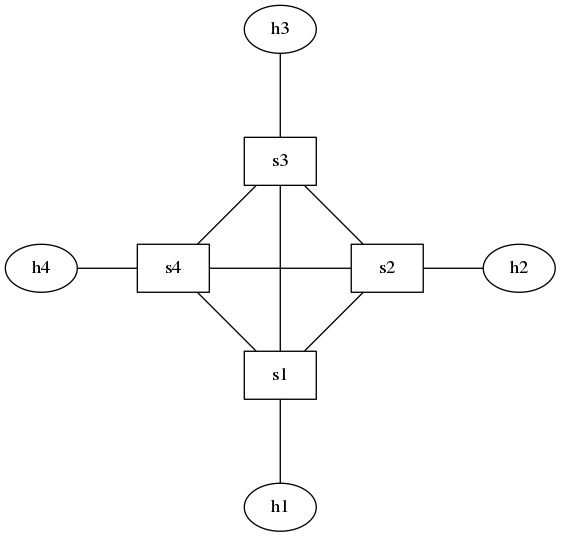
\includegraphics[width=0.40\textwidth]{img/4node.png}
	\caption{Топология <<Ромб>>.}
	\label{pic:4node}
\end{figure}

\begin{figure}[h!]
	\centering
	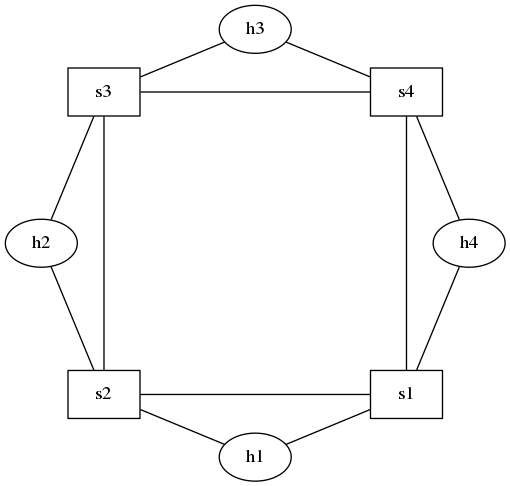
\includegraphics[width=0.40\textwidth]{img/double.png}
	\caption[russian]{Топология <<Двойное резервирование>>.}
	\label{pic:double}
\end{figure}

\begin{figure}[h!]
	\centering
	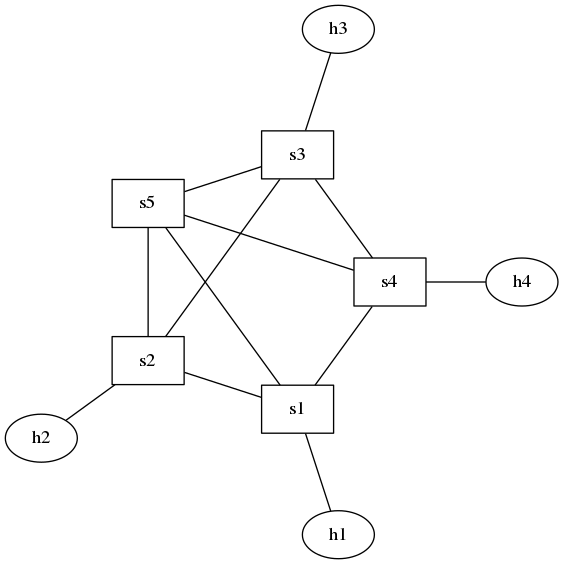
\includegraphics[width=0.40\textwidth]{img/5node.png}
	\caption{Топология <<add Название>>.}
	\label{pic:5node}
\end{figure}

В исследовании используется рекомендованное экспертами в области вычислительных реального времени число виртуальных каналов равное 100.

\subsection{Накладываемые ограничения} \label{subsec:limits}
Процесс реконфигурации сети влечёт за собой потери пакетов, увеличение задержек и джиттеров. Чем быстрее будет производится смена конфигурации, тем меньшее воздействие этот процесс окажет на трафик абонентов бортовой системы. В рамках данного экспериментального исследования будем опираться на временные ограничения, принятые в вычислительных системах реального времени. Как упоминалось в разделе~\ref{sec:scheme}, в сетях FC-AE-ASM-RT на смену конфигурации отводится 40мс. При этом будем учитывать оценки на время, прошедшее с момента отправки последнего управляющего правила до момента его применения в таблице коммутации:

С учётом вышесказанного в качестве итогового времени, отводимого на реконфигурацию примем addмс.
\subsection{Исследование свойств алгоритма}
\subsubsection{Методика исследования}
Исследование свойств алгоритма производится по следующей схеме:
\begin{enumerate}
	\item Для каждого класса данных генерируется соответствующий ему набор виртуальных каналов.
	\item Для каждого набора виртуальных каналов:
	\begin{enumerate}
		\item Запускается приложение, содержащее алгоритм реконфигурации.
		\item Запуск инициирует построение начальных маршрутов виртуальных каналов.
		\item Собирается статистика по количеству виртуальных каналов, проходящих через каждый элемент сети.
		\item Выбирается элемент сети, через который проходит наибольшее число виртуальных каналов, и имитируется его поломка.
		\item Поломка инициирует запуск алгоритма реконфигурации.
		\item По завершению алгоритм выдаёт информацию об успешности и этапе завершения, а так же времени работы.
	\end{enumerate}
	\item Предполагается, что время работы алгоритма занимает не более 70\% от всего времени, заложенного на реконфигурацию.
	\item По полученным характеристикам делается вывод о возможности использования алгоритма в рамках подхода к передаче данных в реальном времени.
\end{enumerate}
 
\subsubsection{Результаты}
Характеристики компьютера, на котором производилось исследование:
\begin{itemize}
	\item Процессор -- Intel Core i7, тактовая частота 1.90 ГГц.
	\item Оперативная память -- 4 ГБ.
\end{itemize}

Результаты исследования свойств алгоритма реконфигурации виртуальных каналов приведены в addПриложение (см. таблицу addТаблица).

Максимальное время работы алгоритма – addмс. Данные показатели времени достигаются, если алгоритм вынужден выполнить дополнительный этап. Следует отметить, что выполнение дополнительного этапа произошло в add\% случаев. Как правило алгоритм завершает работу на базовом этапе. При таком варианте выполнения время завершения алгоритма не превышает addмс. Время работы алгоритма, не превысило 70\% от времени, отведённого на реконфигурацию. То, как данная величина соотносится со временем, затрачиваемым на применение полученных изменений в сети, будет продемонстрировано в разделе~\ref{subsec:approbation}.

Алгоритм не смог построить новую систему виртуальных каналов при add. Это объясняется тем, что add.

\subsection{Апробация разработанного подхода динамической реконфигурации сети} \label{subsec:approbation}
\subsubsection{Конфигурация экспериментальной системы}
Система апробации представляет собой виртуальную среду, имитирующую
функционирование:
\begin{enumerate}
	\item Контроллера сети.
	\item Набора коммутаторов.
	\item Абонентов сети, формирующих потоки данных с заданными характеристиками.
\end{enumerate}

Виртуальная среда разворачивается на основе операционной системы Ubuntu 16.04,
на которой установлены следующие компоненты:
\begin{enumerate}
	\item Runos -- ПКС-контроллер \cite{runos}.
	\item Ofsoftswitch13 -- программный коммутатор, поддерживающий OpenFlow 1.3 \cite{ofsoftswitch}.
	\item Mininet -- средство имитирующее работу сети \cite{mininet}.
\end{enumerate}

\subsubsection{Сценарии апробации}

Для апробации предложенного подхода к передаче данных в реальном времени был выбран набор сценариев, основывающийся на том, какие элементы сети могут выйти из строя. 

Рассматривается выход из строя:
\begin{enumerate}
	\item Коммутатора.
	\item Физической линии, соединяющей два коммутатора.
	\item Физической линии, соединяющей абонента с коммутатором.
	\item Порта абонента или коммутатора.
\end{enumerate}

Дополнительно к этому рассматриваются сценарии кратных последовательных во времени выходов из строя элементов сети.

Сценарии разрыва физической линии между коммутаторами и выхода из строя соответствующих портов производятся на всех топологиях. Оставшиеся сценарии могут быть выполнены только на топологиях <<Двойное резервирование>> и <<add Название>> (см. рисунки~\ref{pic:double} и~\ref{pic:5node}). Отказ портов практически ничем не отличается от отказа соответствующих им физических линий. Поэтому в таблице результатов данные по таким сценариям представлены не будут.

\subsubsection{Методика апробации}
Апробация работы алгоритма реконфигурации в рамках предложенного подхода состоит из трёх этапов:
\begin{enumerate}
	\item Формирование набора тестовых прецедентов.
	\item Проведение экспериментов на тестовых прецедентах.
	\item Анализ результатов.
\end{enumerate}

Тестовые прецеденты формируются выбором:
\begin{itemize}
	\item сценария апробации;
	\item класса исходных данных с доступной для выбранного сценария топологией сети.
\end{itemize}

На этапе проведения экспериментов производится запуск каждого тестового прецедента:
\begin{enumerate}
	\item Формируется соответствующая классу данных конфигурация сети.
	\item Запускается приложение реконфигурации.
	\item Запускается виртуальная тестовая среда, имитирующая поведение сети.
	\item Запуск приложения инициирует построение начальных маршрутов виртуальных каналов.
	\item Запуск тестовой среды инициирует отправку и прием потоков данных абонентами, а так же сбор статистики по этим потокам данных.
	\item Средствами тестовой среды запускается сценарий апробации.
	\item Соответствующая сценарию поломка инициирует запуск алгоритма реконфигурации.
	\item По завершению алгоритм выдаёт информацию о времени, затраченном на применение изменений в сети.
	\item Происходит сворачивание тестовой среды, инициирующее обработку собранной статистики по потокам данных.
\end{enumerate}

На этапе анализа результатов для каждого тестового прецедента:
\begin{enumerate}
	\item Проверяется факт восстановления трафика по завершению выполнения сценария.
	\item Анализируется время, затраченное на применение изменений в сети.
	\item Анализируется число потерянных в ходе реконфигурации пакетов.
	\item Задержки и джиттеры, полученные в период реконфигурации сравниваются с эталонными задержками, полученными в штатном режиме.
	\item Делается вывод об успешности работы приложения реконфигурации в рамках предложенного сценария.
\end{enumerate}

\subsubsection{Результаты}

Результаты апробации работы алгоритма в рамках приложения, реализующего подход к передаче данных в условиях реального времени в ПКС, приведены в addПриложение (см. таблицу addТаблица).

Джиттеры и задержки потоков данных, виртуальные каналы которых участвовали в реконфигурации, отличались от эталонных не более, чем на addмс и addмс соответственно. Данное отклонение лежит в рамках допустимого. Джиттеры и задержки прочих потоков данных не изменились.

Максимальное время затраченное на процесс реконфигурации удовлетворяет наложенным в разделе~\ref{subsec:limits} ограничениям. Потери пакетов составили add. При этом потоки, маршруты виртуальных каналов которых не проходили через сбойные элементы, затронуты не были.

Отказы от построения новых виртуальных каналов были получены на тех же классах данных, что и при исследовании свойств алгоритма.

Было проверено несколько сценариев кратного последовательного во времени выхода из строя элементов сети. Максимальное число последовательных поломок, после которых восстанавливалась работоспособность системы, составило add. Отказы от восстановления работы сети после очередной поломки были обусловлены исключительно отсутствием путей между абонентами или нехваткой пропускных способностей.

\subsection{Выводы}
Проведенное экспериментальное исследование продемонстрировало, что:
\begin{itemize}
	\item основные характеристики алгоритма соответствуют ожидаемым;
	\item алгоритм успешно функционирует в рамках приложения реконфигурации, работающего в виртуальной среде, имитирующей сеть ПКС;
	\item соблюдаются ограничения на характеристики качества обслуживания абонентских потоков данных при реконфигурации сети с использованием предложенного алгоритма.
\end{itemize}

Исследование и апробация показали, что предложенный алгоритм реконфигурации виртуальных каналов способен работать в составе приложения, реализующего подход к передаче данных в реальном времени в ПКС. Алгоритм успешно осуществляет поиск новых маршрутов для виртуальных каналов при выходе из строя различных элементов сети. Апробация показала работоспособность разработанного приложения, осуществляющего функции реконфигурации и мониторинга, и реализуемого им подхода. Время, затраченное на осуществление реконфигурации, не превосходит ограничений, заданных в существующих системах реального времени.

\section*{Заключение}
\addcontentsline{toc}{section}{Заключение}
выводы из всей работы, решенные задачи, возможные направления дальнейших исследований темы 

\renewcommand{\bibname}{Список литературы}
\addcontentsline{toc}{section}{\bibname}
\bibliographystyle{unsrt}
\begin{thebibliography}{}
	\bibitem{afdx}
	AFDX / ARINC 664 Tutorial (1500-049) // Condor Engineering, Inc. -- 2005.
	\bibitem{fcaert}
	Fibre Channel Arbitrated Loop (FC-AL) // working draft proposal American National Standard for Information Technology. 1995. 98 p.
	\bibitem{sdn}
	Software-Defined Networking: The New Norm for Networks // Open Networking Foundation. -- 2012. [PDF] (https://www.opennetworking.org/images/stories/downloads/sdn-resources/white-papers/wp-sdn-newnorm.pdf)
	\bibitem{vlsdn}
	Balashov V., Kostenko V., Ermakova T. An SDN-based approach to design of onboard real-time networks // Modern Network Technologies, MoNeTec-2018. -- Moscow, 2018. -- P. 16-22.
	\bibitem{vdovin}
	Vdovin P. M., Kostenko V. A. Organizing message transmission in AFDX networks // Programming and Computer Software. -- 2017. -- Vol. 43, No 1. -- P. 1-12. [DOI] (https://link.springer.com/article/10.1134\%2FS0361768817010078).
	\bibitem{meter}
	Efimushkin, T. Ledovskikh, D. Korabelnikov, D. Iazykov. Perfomance assurance in Software-Defined Networks // « Intellect Telecom» JSC.
	\bibitem{openflow}
	ONF OpenFlow Switch Specification, Version1.3.0 [PDF] (https://www.opennetworking.org/images/stories/downloads/sdn-resources/onf-specifications/openflow/openflow-spec-v1.3.0.pdf)
	\bibitem{ofsoftswitch}
	CPqD F. Openflow 1.3 software switch [HTML] (http://www.cpqd.github.io/ofsoftswitch13/).
	\bibitem{fakevlsdn}
	Cevher S. et al. A Fault Tolerant Software Defined Networking Architecture for Integrated Modular Avionics // 37th Digital Avionics Systems Conference (DASC). -- IEEE, 2018. -- С. 1-9.
	\bibitem{alg1}
	Al Sheikh A. et al. Optimal design of virtual links in AFDX networks // Real-Time Systems. -- 2013. -- Т. 49. -- No 3. -- P. 308-336.
	\bibitem{vdovinalg}
	Вдовин П. М. Инструментальная система проектирования сетей AFDX // Труды Московского физико-технического института. -- 2015. -- Т. 7. -- №. 2. -- С. 131-137.
	\bibitem{dejkstra}
	Golden B. Shortest-path algorithms: A comparison // Operations Research. -- 1976. -- Т. 24. -- №. 6. -- С. 1164-1168.
	\bibitem{kshort}
	Yen J. Y. Finding the k shortest loopless paths in a network // Management Science. -- 1971. -- Т. 17. -- No 11. -- P. 712-716.
	\bibitem{monitor1}
	Ochoa Aday L., Cervelló Pastor C., Fernández Fernández A. Current trends of topology discovery in OpenFlow-based software defined networks. -- 2015.
	\bibitem{monitor2}
	Pakzad F. et al. Efficient topology discovery in software defined networks // 2014 8th International Conference on Signal Processing and Communication Systems (ICSPCS). -- IEEE, 2014. -- С. 1-8.
	\bibitem{cpp}
	Orozco J. D., Santos R. M. Real-Time Operating Systems and Programming Languages for Embedded Systems. // INTECH Open Access Publisher. -- 2012.
	\bibitem{nox}
	Gude N. NOX: towards an operating system for networks // ACM SIGCOMM Computer Communication Review. -- 2008. -- Т. 38. -- №. 3. -- P. 105-110.
	\bibitem{runos}
	Shalimov A. et al. The Runos OpenFlow Controller // Software Defined Networks (EWSDN), 2015 Fourth European Workshop on. -- IEEE, 2015. -- С. 103-104.
	\bibitem{mininet}
	Oliveira R. L. S. Using mininet for emulation and prototyping software-defined networks // Communications and Computing (COLCOM) -- 2014. -- P. 1-6
\end{thebibliography}

\end{document}